\section{Results}
\label{sec:results}

\subsection{Differential Model}
\label{subsec:basicmod}

\begin{figure}[H]
\captionsetup{width=0.6\textwidth}
\centering
    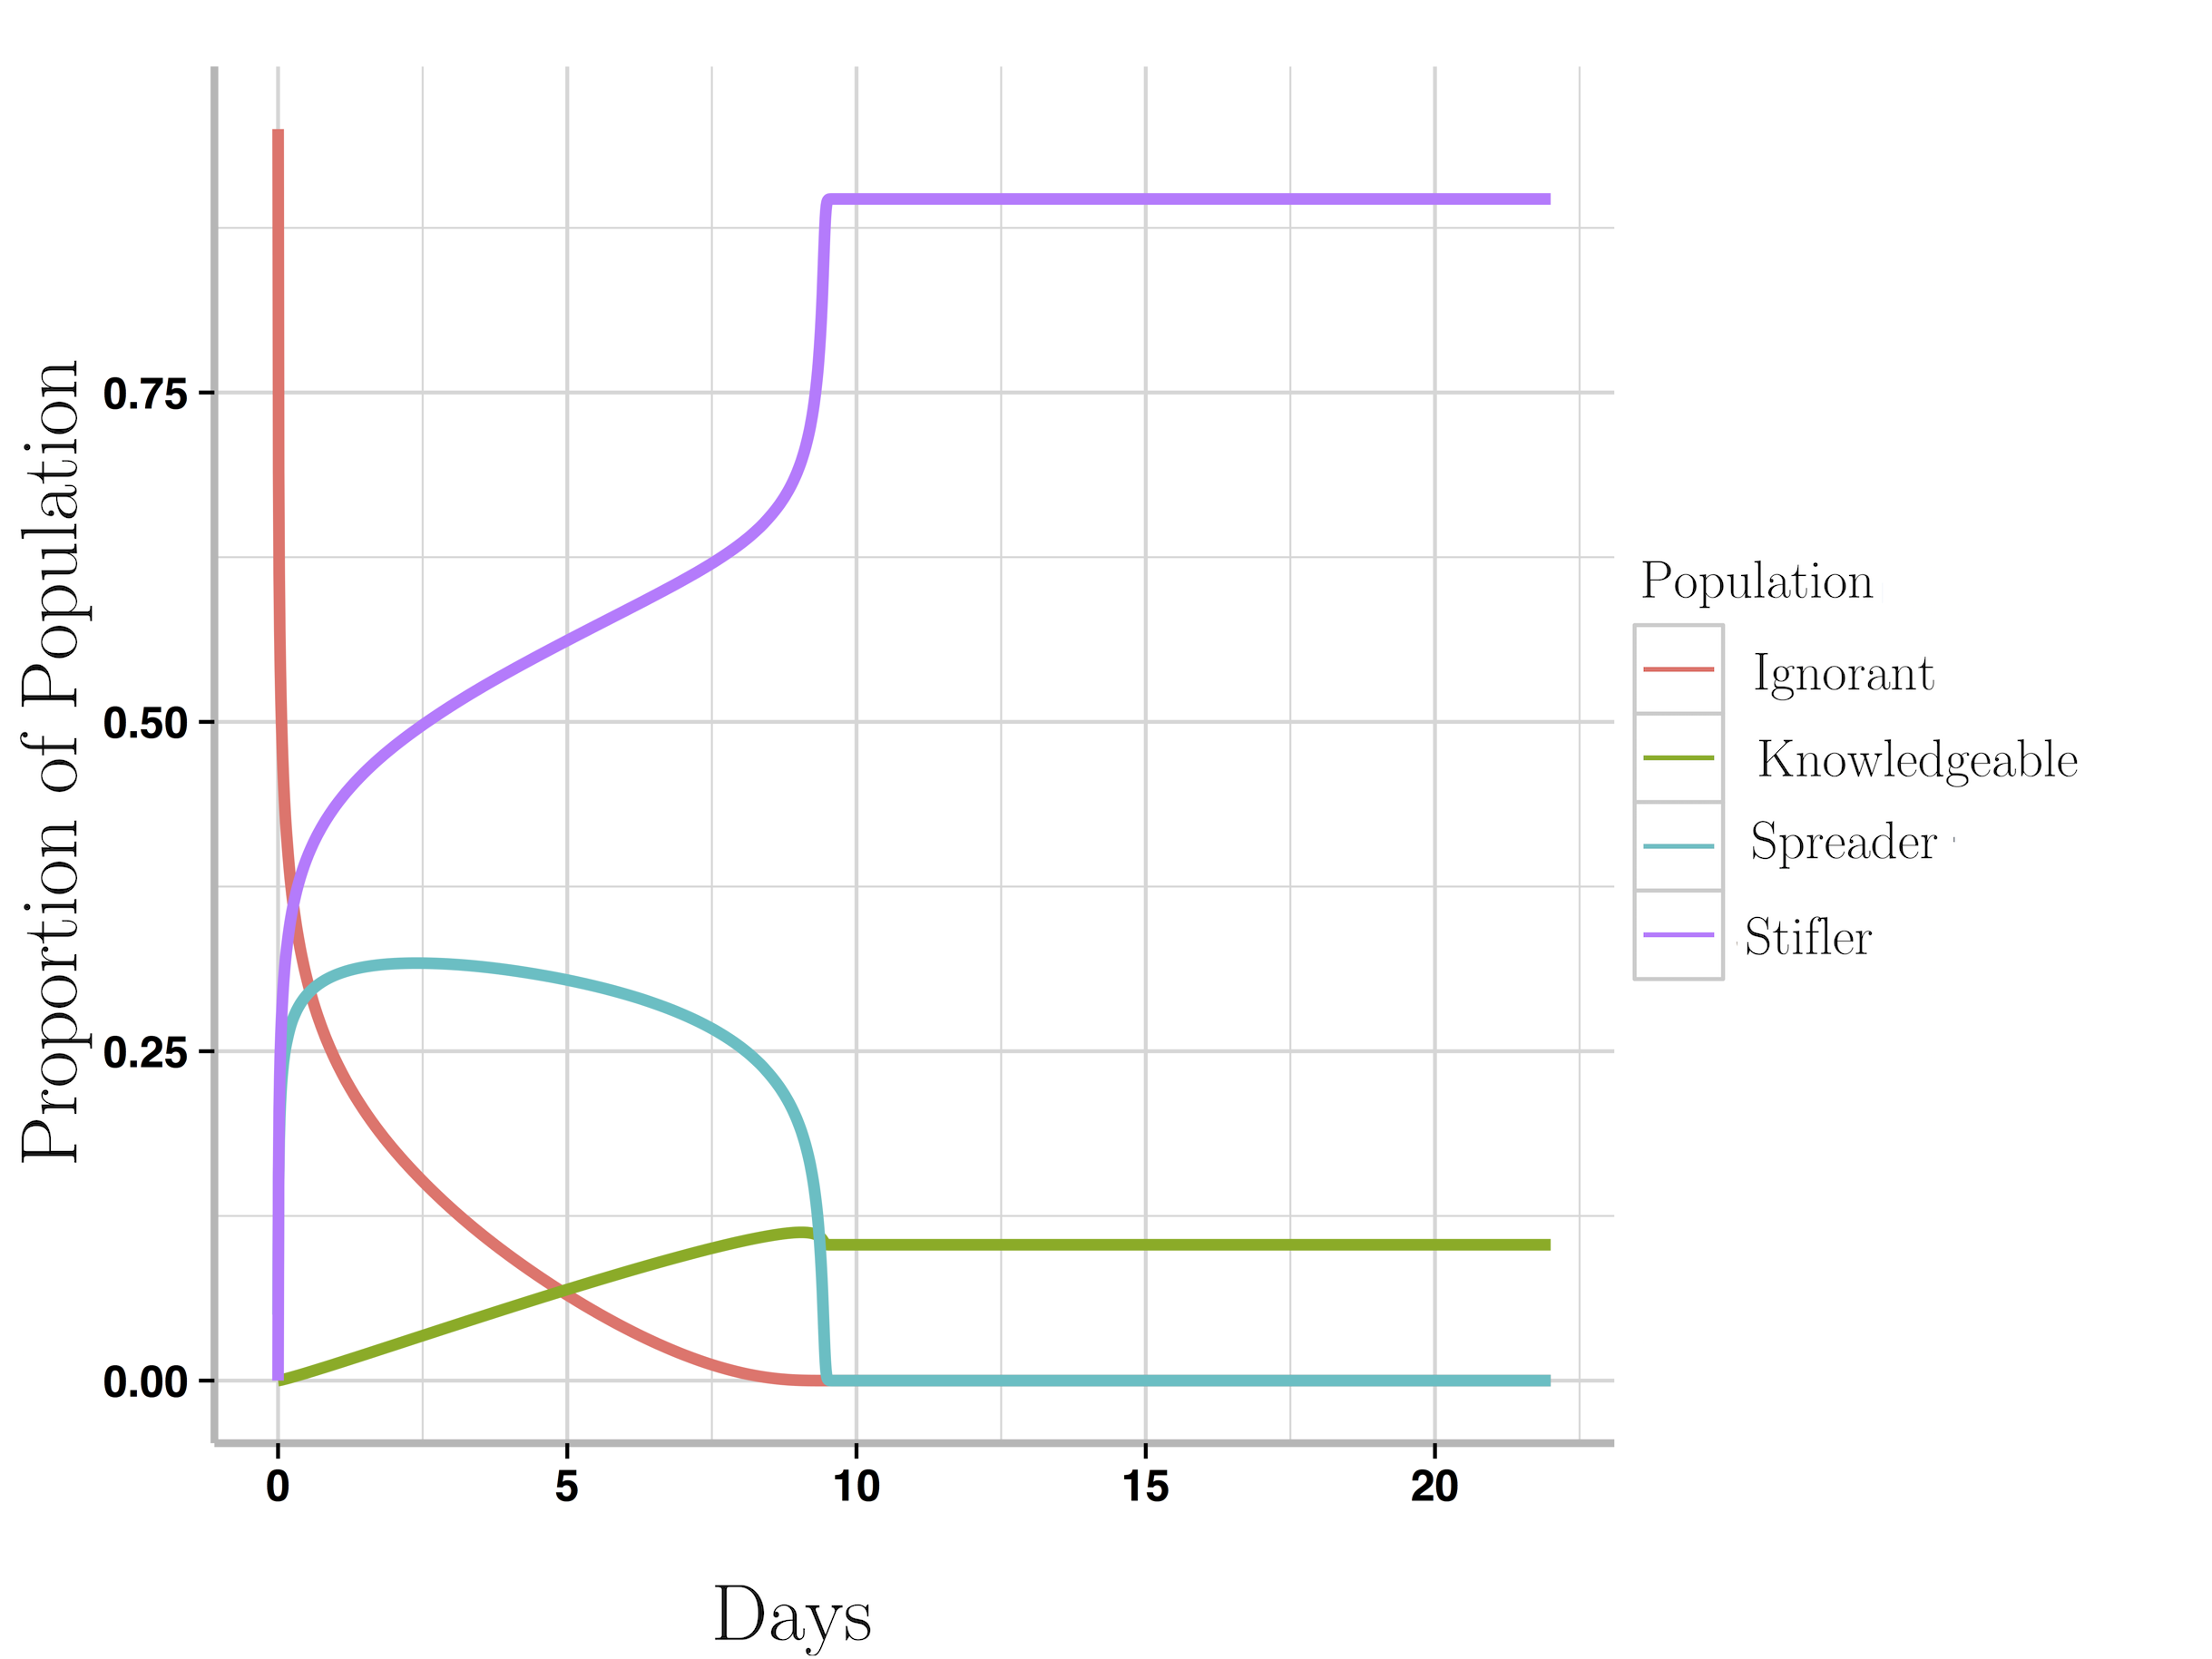
\includegraphics[width=0.7\textwidth]{figures/figure1}
  \caption{Differential model proportions of the population in each class over 22 days.}
\label{fig:figure1}
\end{figure}

For the differential model, as is demonstrated in Figure~\ref{fig:figure1}, the spreader and ignorant populations become negligible by the end of the 22 days, and the knowledgeable and stifler populations stabilize above 0.
The ignorant population declines, as the spreader population initially grows, and then declines as the stifler population grows.
In the differential model, essentially all individuals learn about the rumor.
Varying the parameters impacts how quickly the population hears of the rumor, but not the ignorant and spreader populations.

\begin{figure}[H]
\captionsetup{width=0.8\textwidth}
\centering
    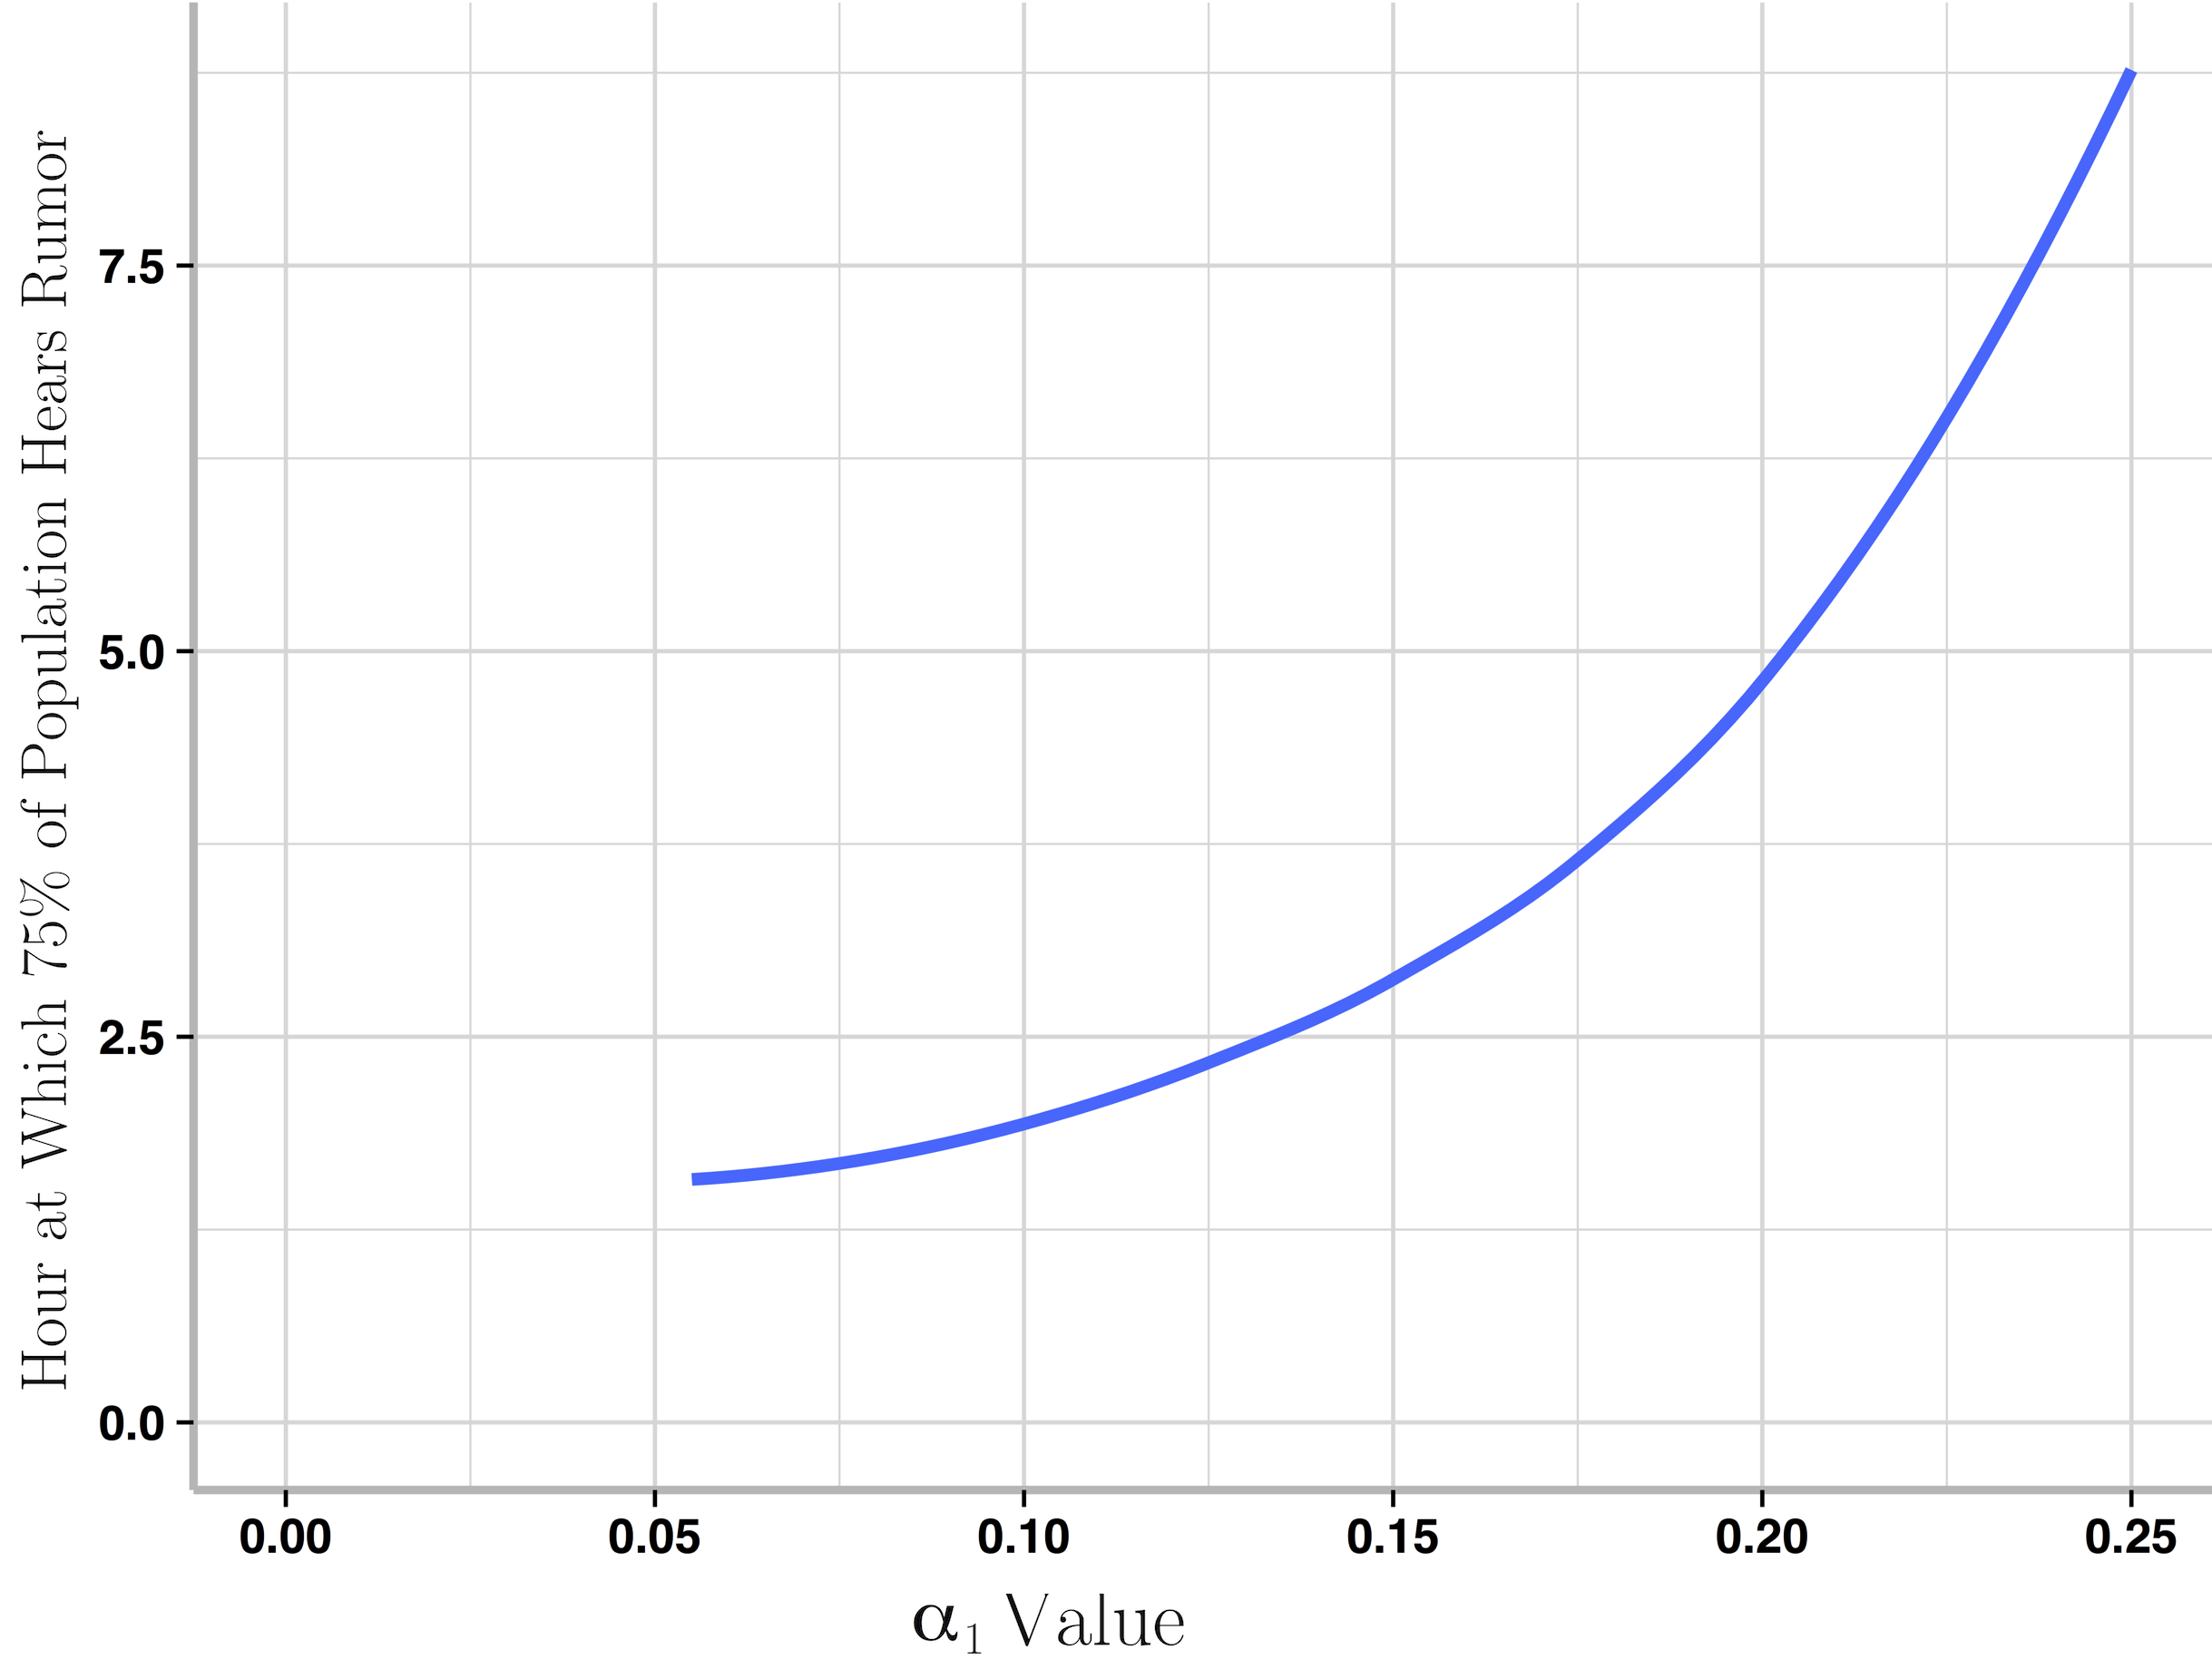
\includegraphics[width=0.7\textwidth]{figures/figure2}
  \caption{Sensitivity analysis of parameter $ \alpha_1 $ (loss of novelty) in the differential model, n.b.\ $ \alpha_2 $ always equaled $ 2 * \alpha_1 $}
\label{fig:figure2}
\end{figure}

\begin{figure}[H]
\captionsetup{width=0.8\textwidth}
\centering
    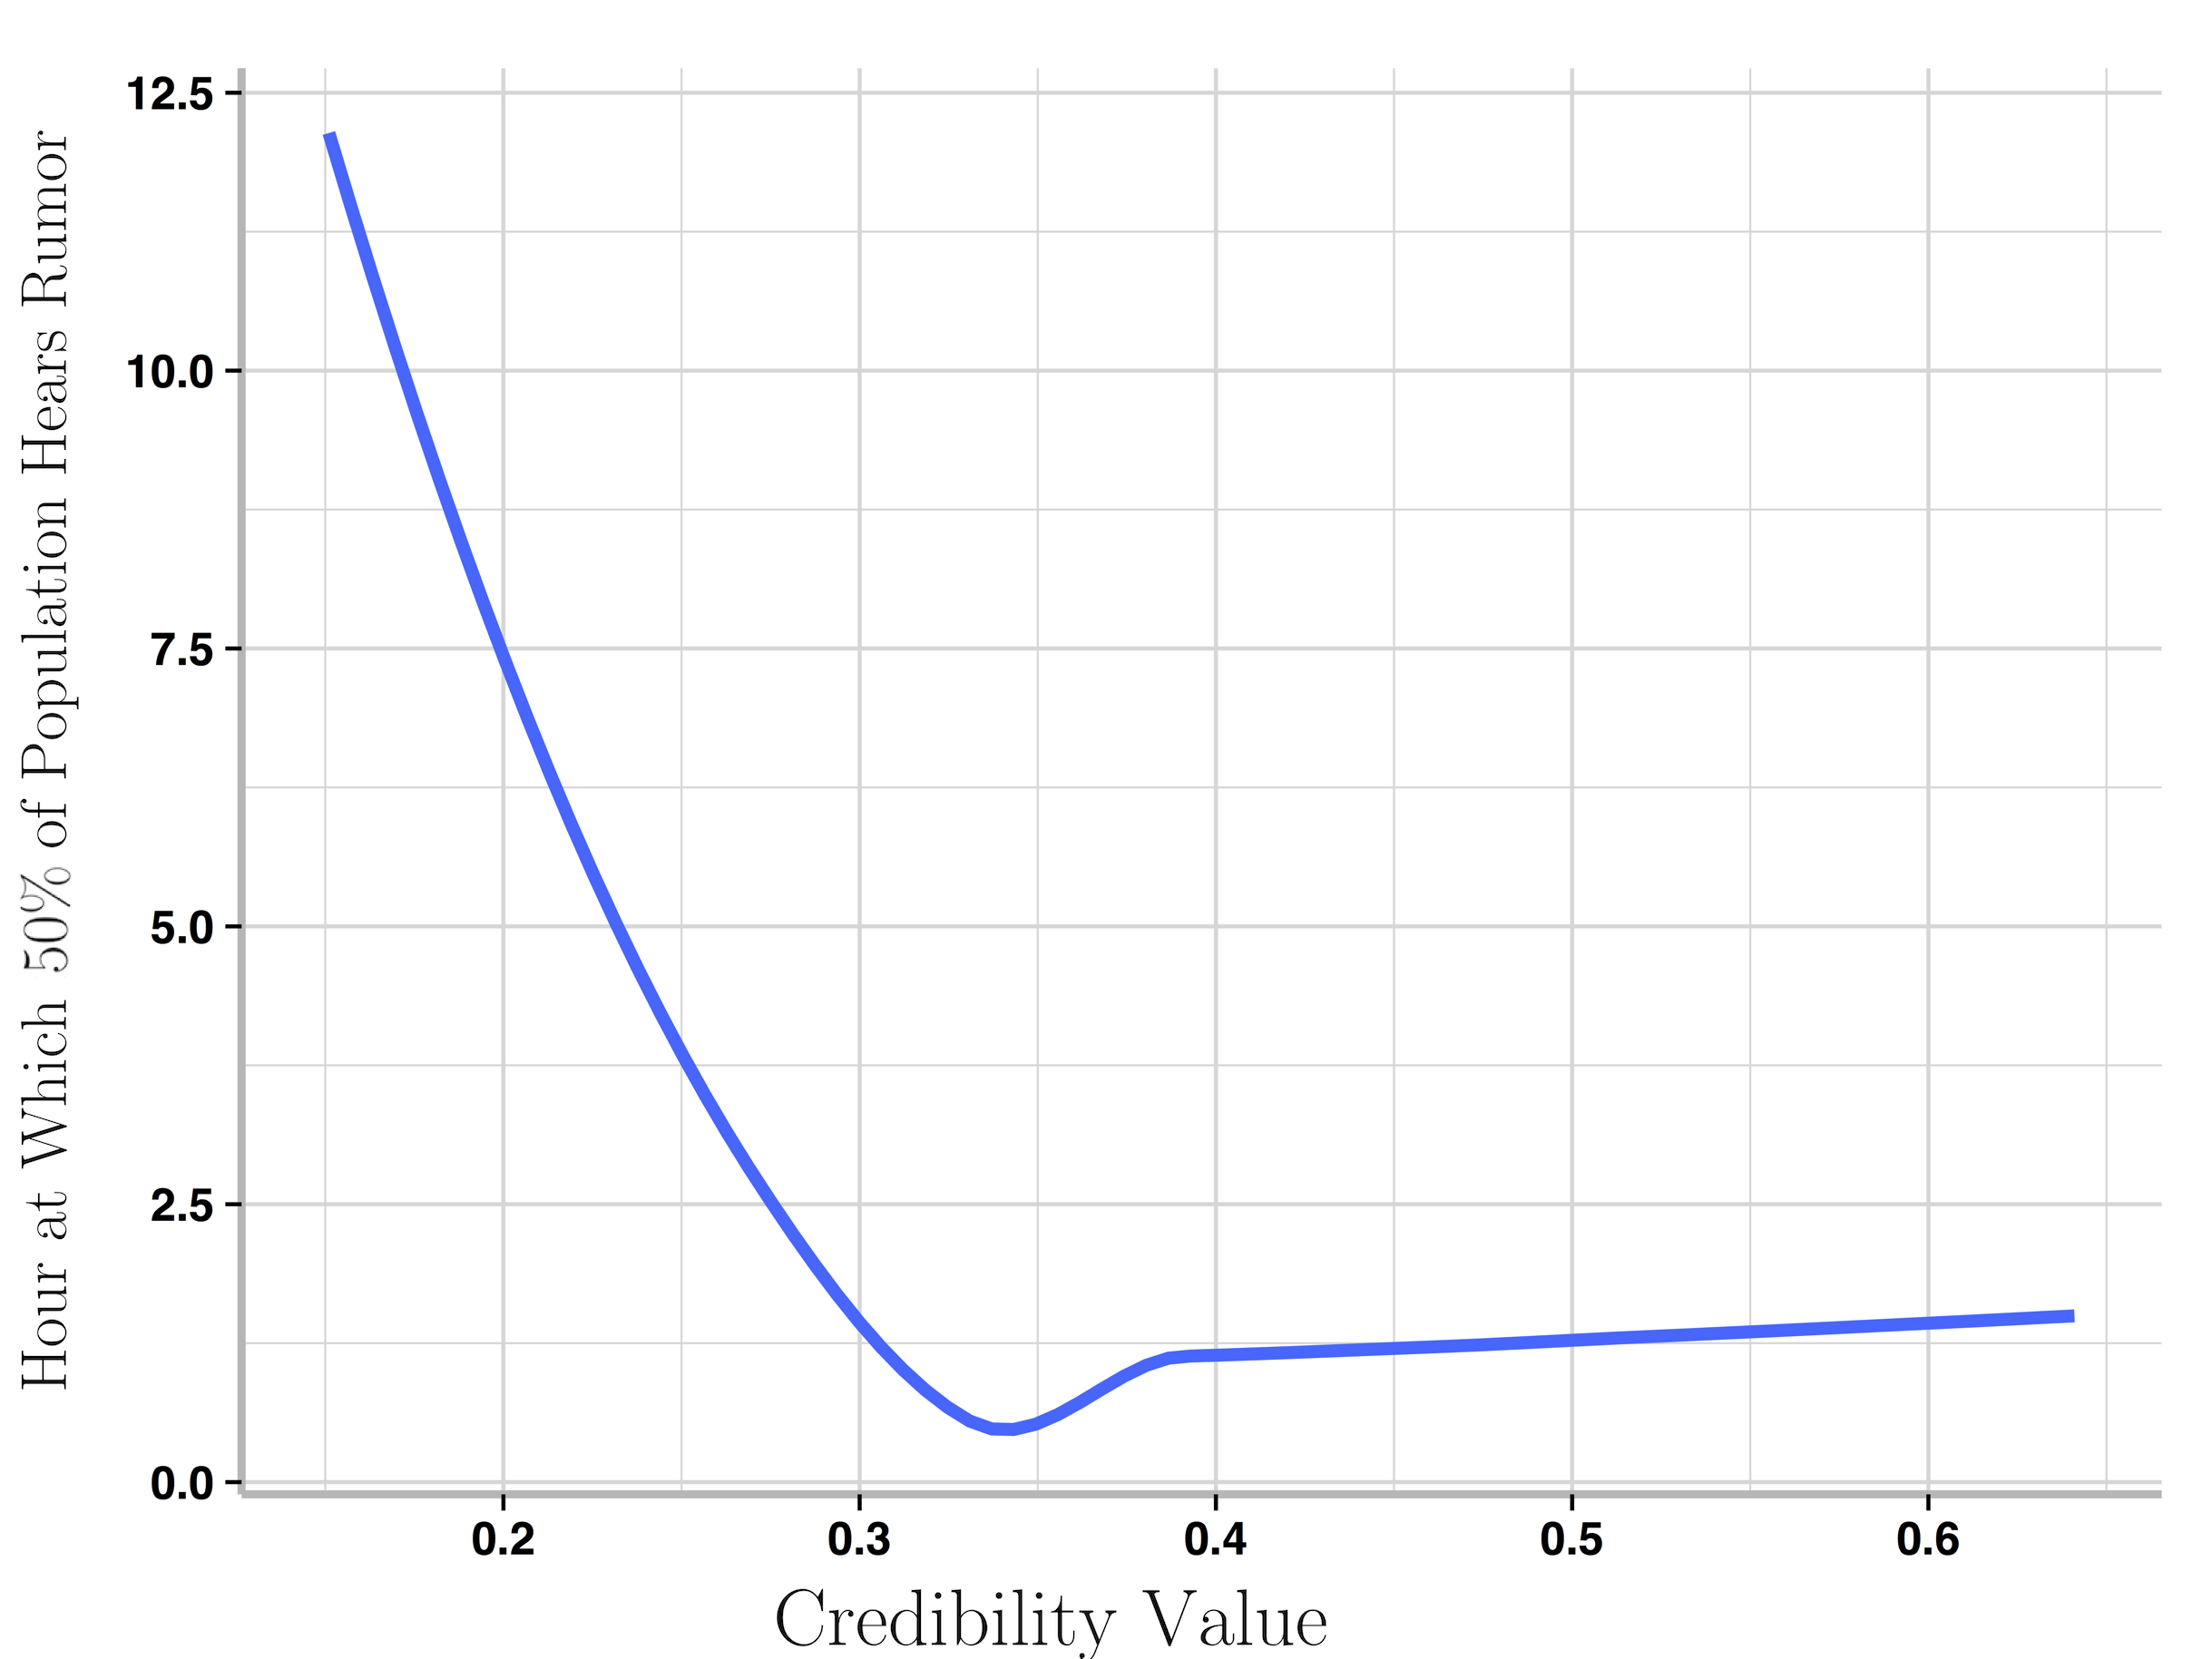
\includegraphics[width=0.7\textwidth]{figures/figure3}
  \caption{Sensitivity analysis of parameter $ c $ (credibility) in the differential model.}
\label{fig:figure3}
\end{figure}

\begin{figure}[H]
\captionsetup{width=0.8\textwidth}
\centering
    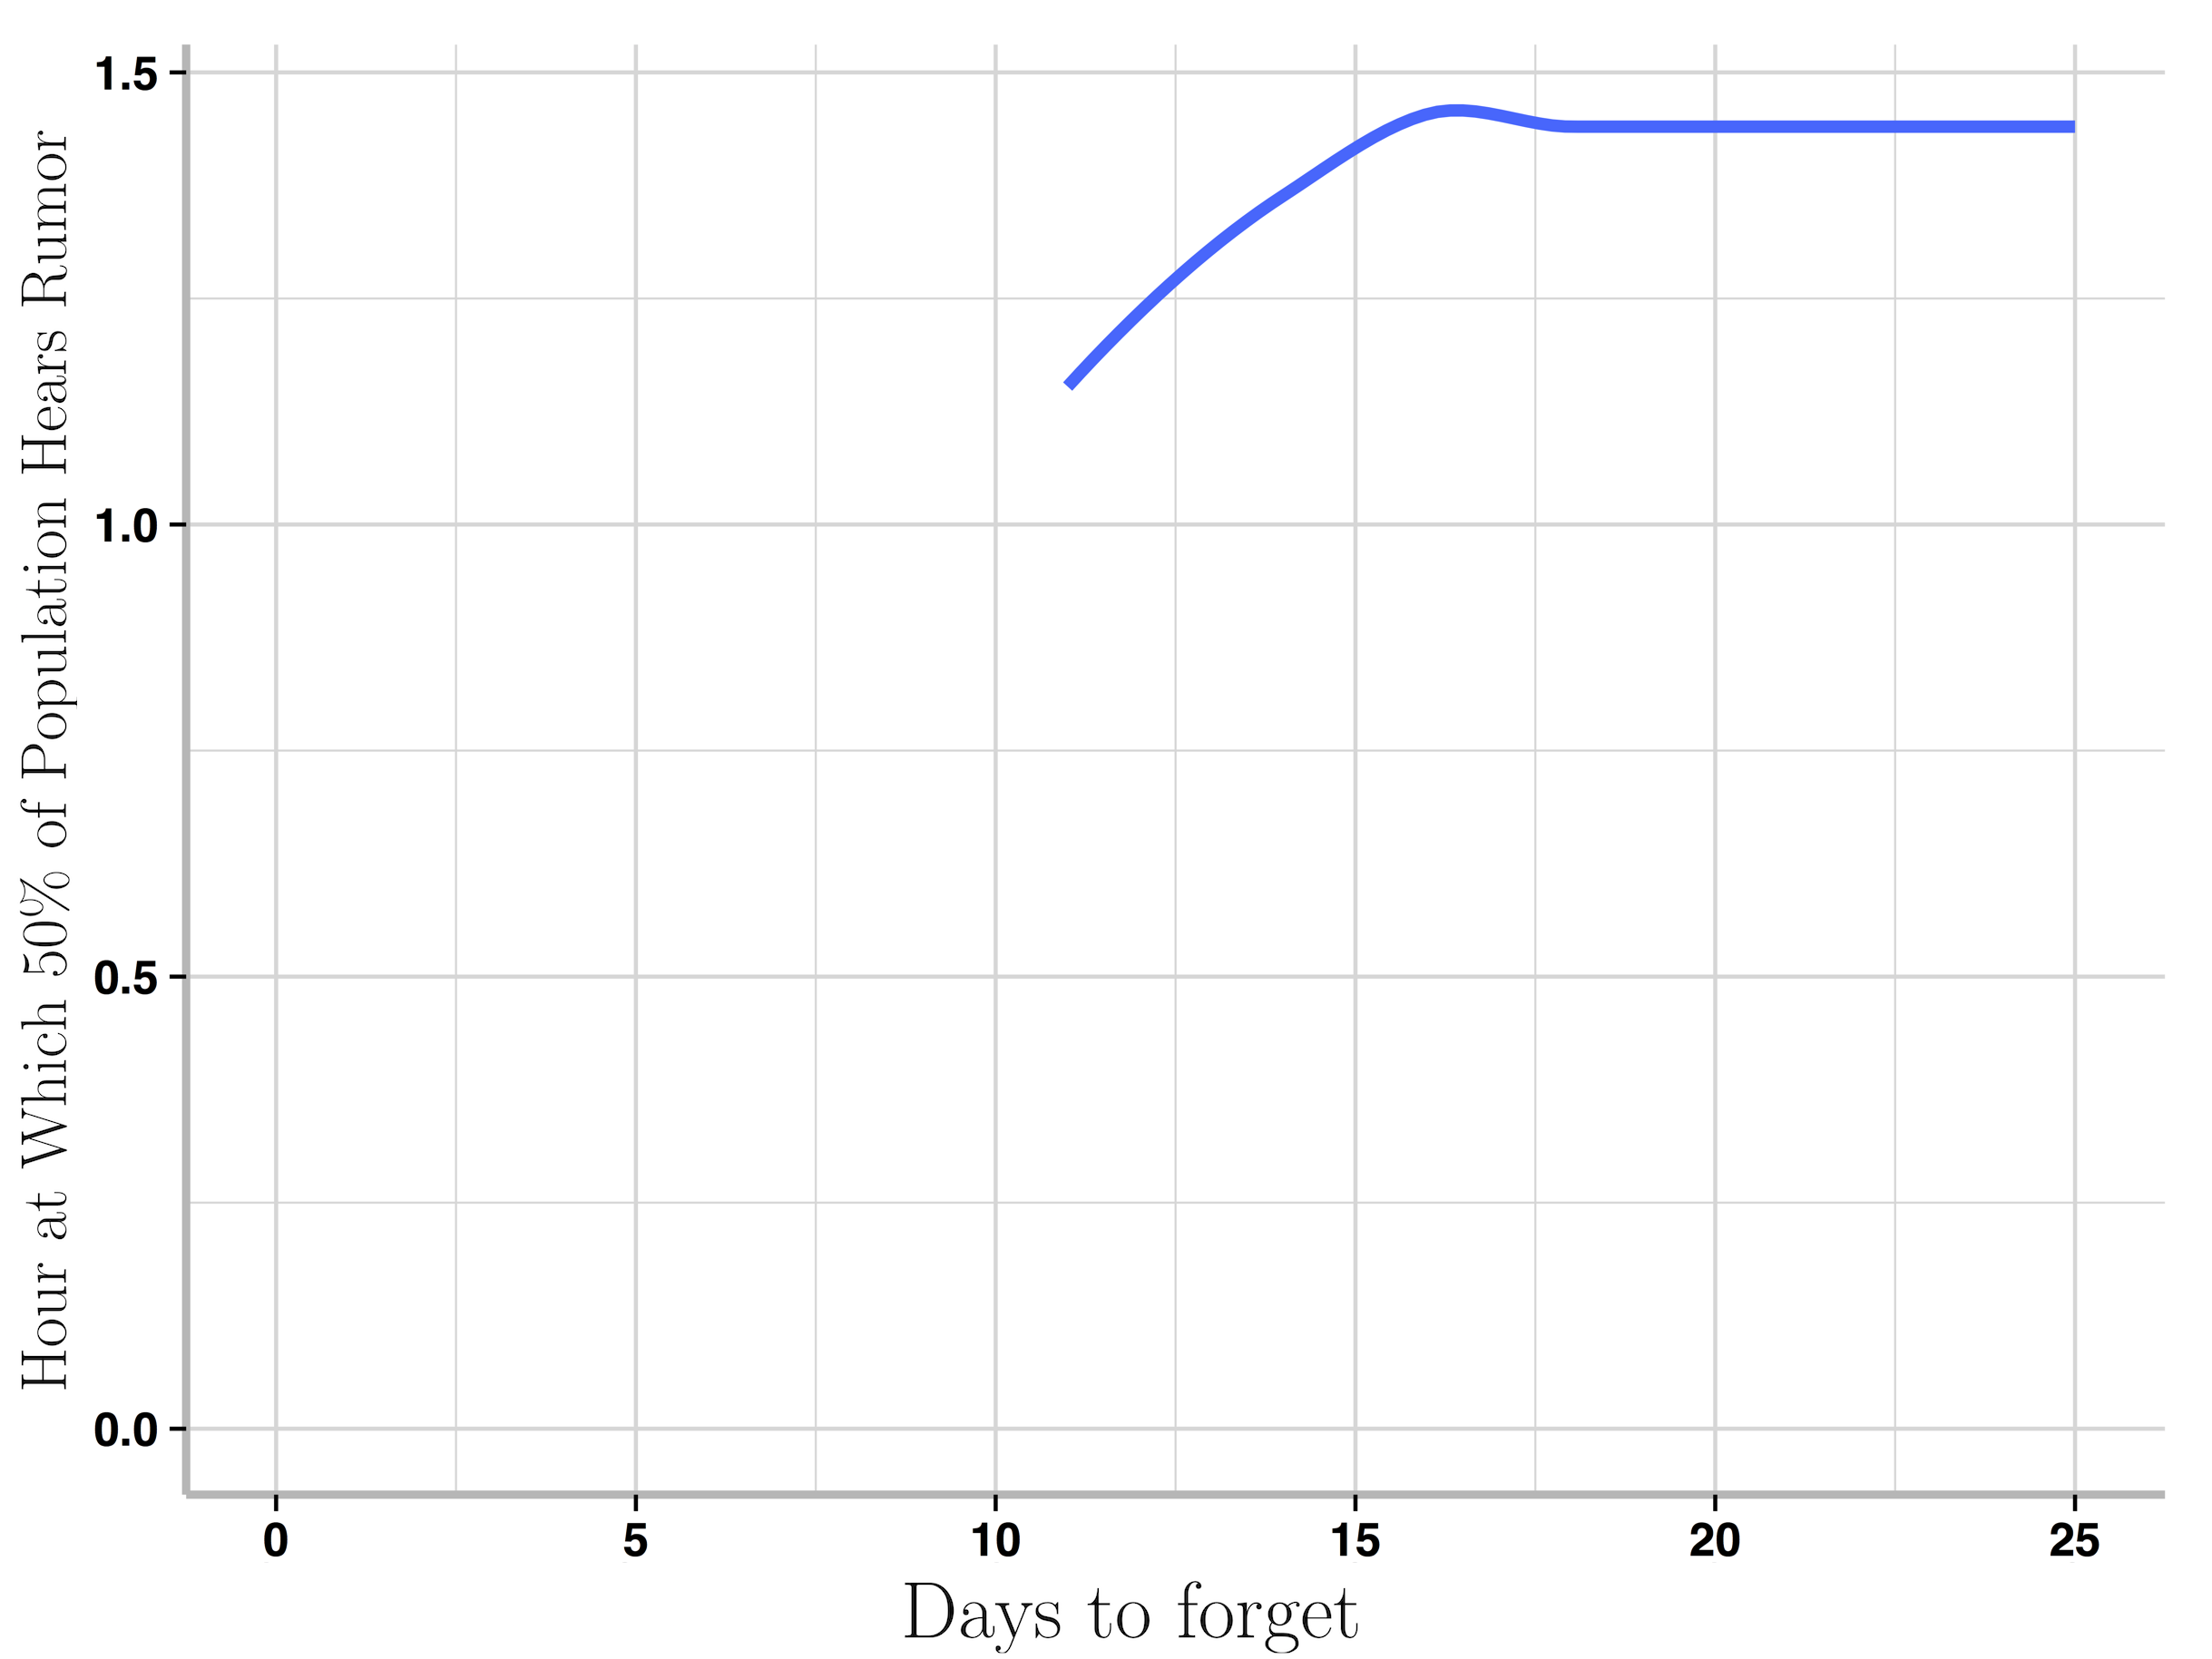
\includegraphics[width=0.7\textwidth]{figures/figure4}
  \caption{Results of the sensitivity analysis of parameter $ d $ (average days to forget) in the differential model.}
\label{fig:figure4}
\end{figure}

Looking at Figures~\ref{fig:figure2},~\ref{fig:figure3}, and~\ref{fig:figure4}, we see can see how changing parameters in the differential model influences the speed at which the rumor travels.
The sensitivity analyses indicate that the rumor travels exponentially slower with increasing $ \alpha $ values, while traveling exponentially faster with increasing credibility values.
The rumor was not particularly sensitive to $ d $, the average days to forget it, but to our surprise, the rumor required more time to travel as $ d $ \textit{increased}.
This effect is probably due to the fact that a shorter $ d $ caused faster movement between populations.

\subsection{Simple, Agent-Based Model}

\begin{figure}[H]
\captionsetup{width=0.8\textwidth}
\centering
    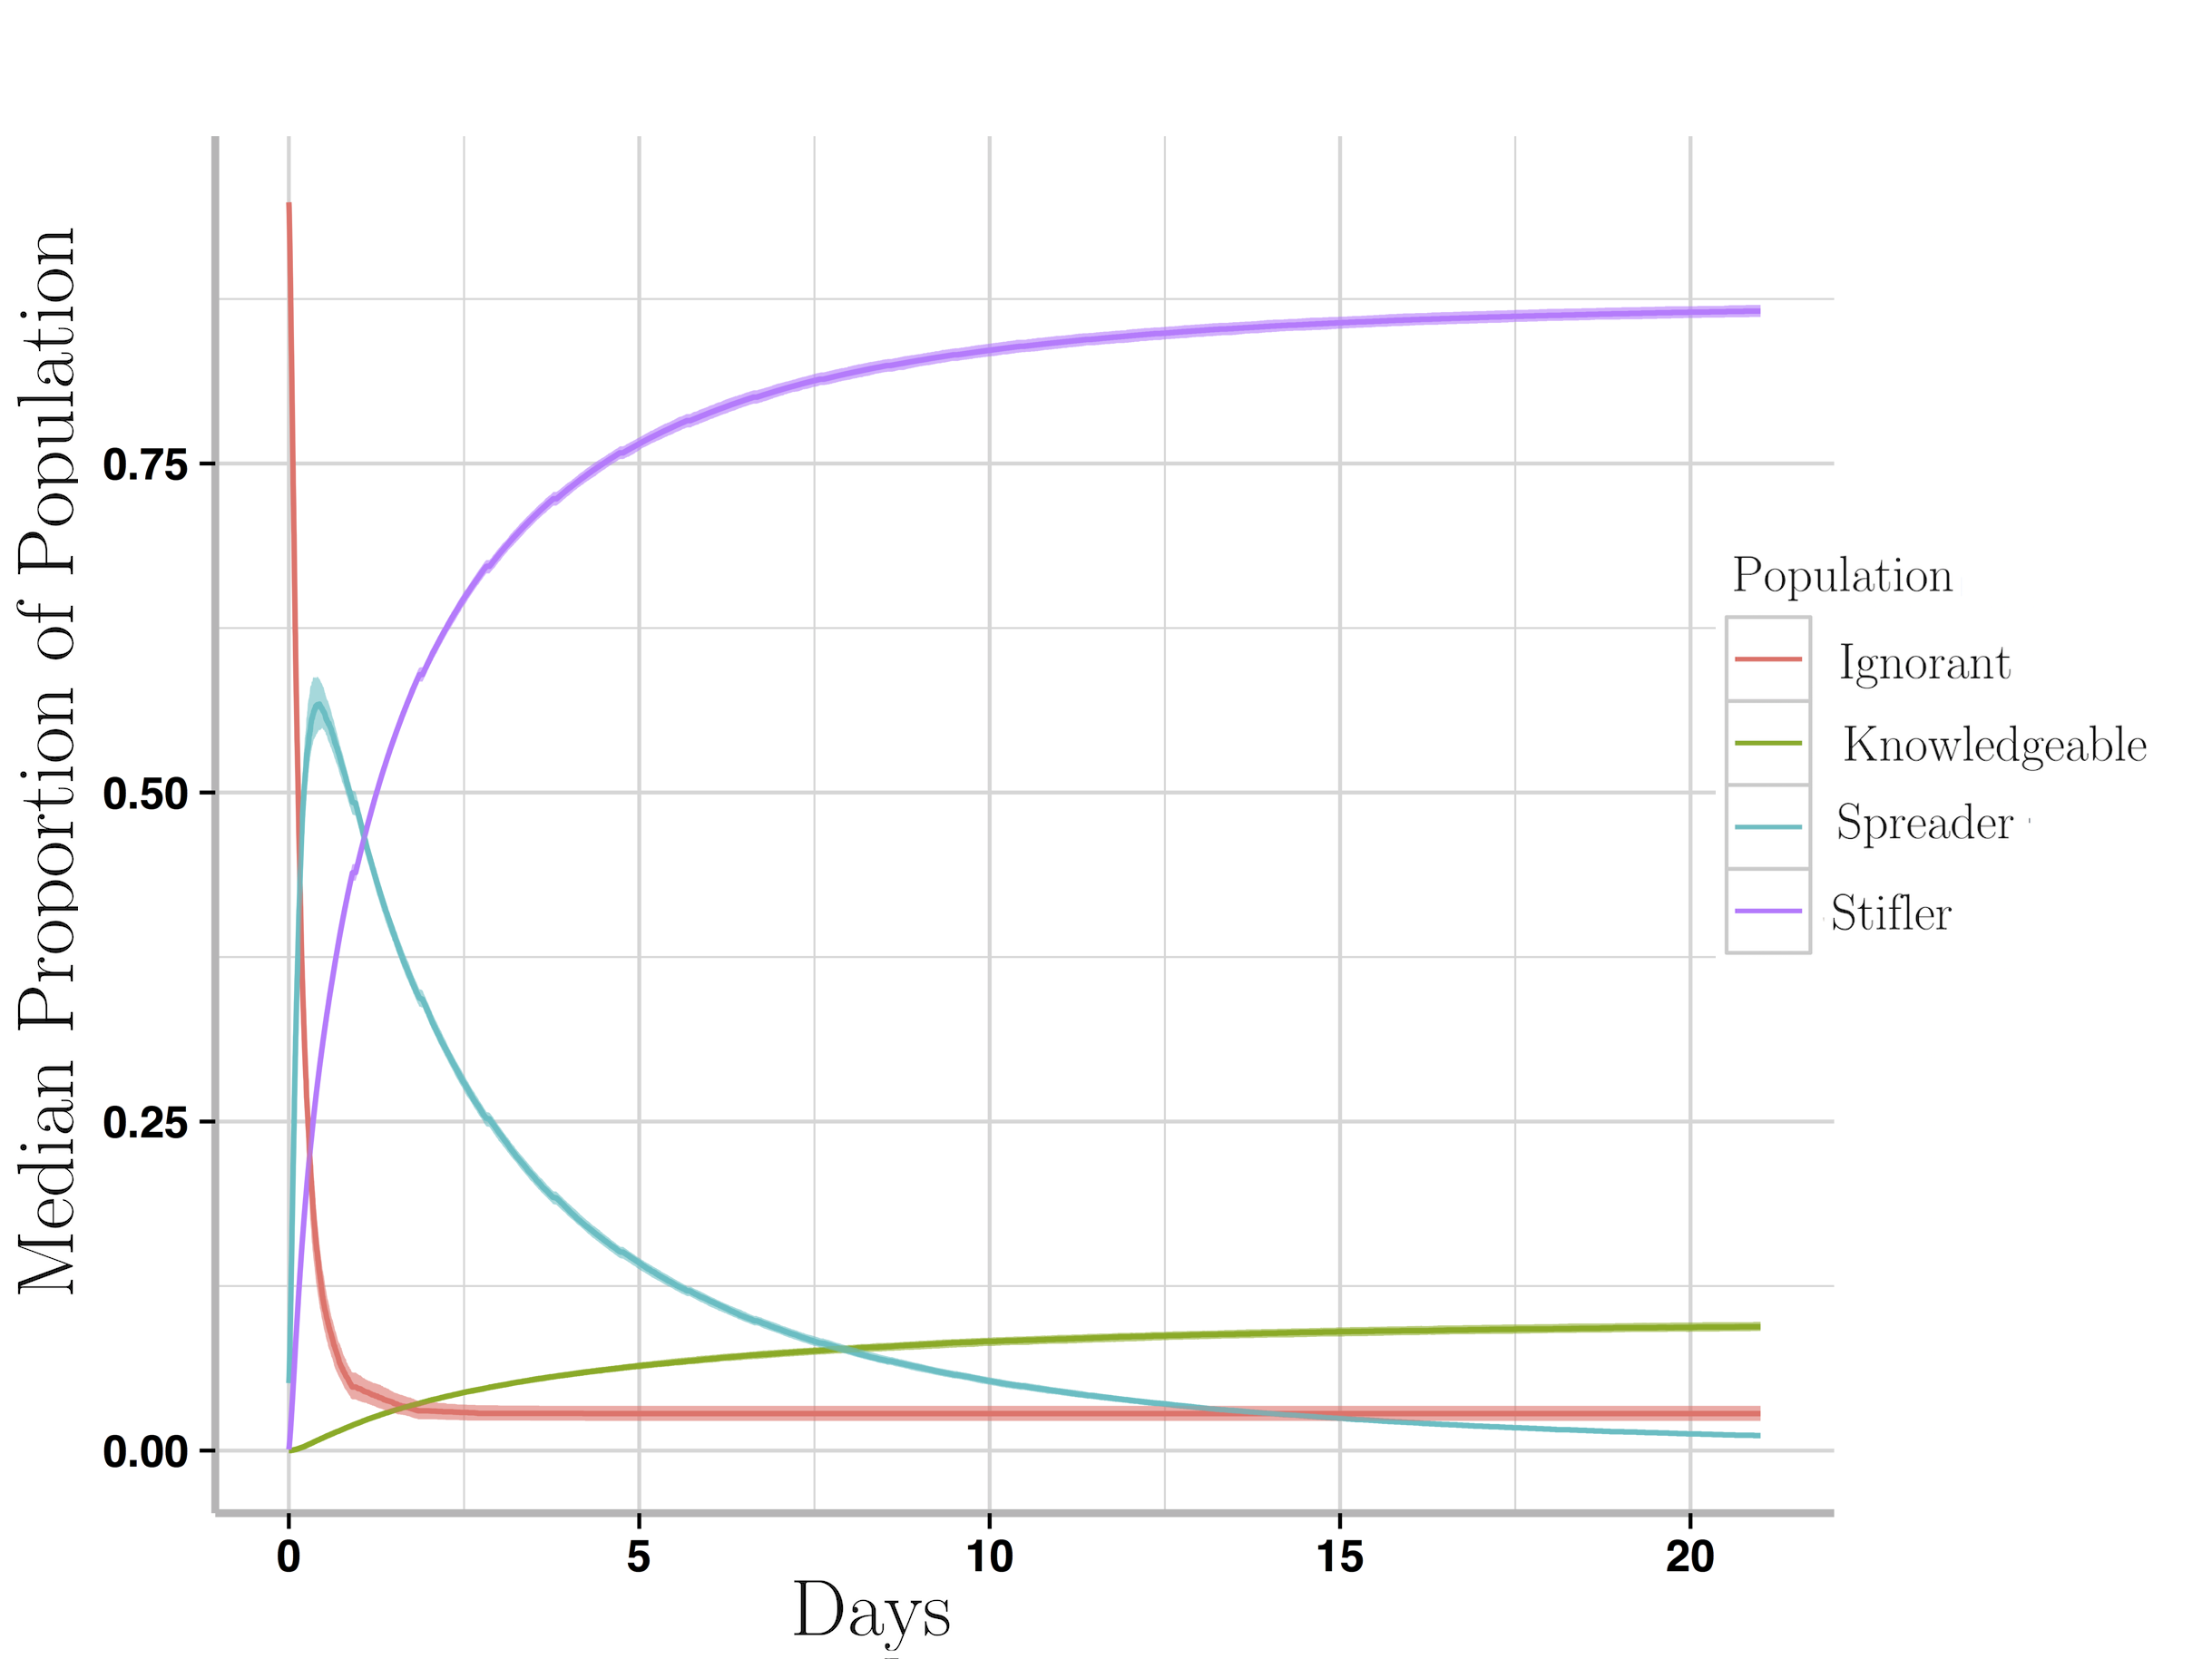
\includegraphics[width=0.7\textwidth]{figures/figure5}
  \caption{Results of the agent-based model.
Solid line indicates median proportion of population across the 400 trials; shadow indicates IQR.}
\label{fig:figure5}
\end{figure}

Analogous to (Figure~\ref{fig:figure1}) for the differential model, we see the average results of the simple, agent-based model.
Interestingly, the dynamics of the rumor's spread are quite different: the slope of the population graphs are more gradual, rather than moving sharply, as in the differential model.

\begin{figure}[H]
\captionsetup{width=0.8\textwidth}
\centering
    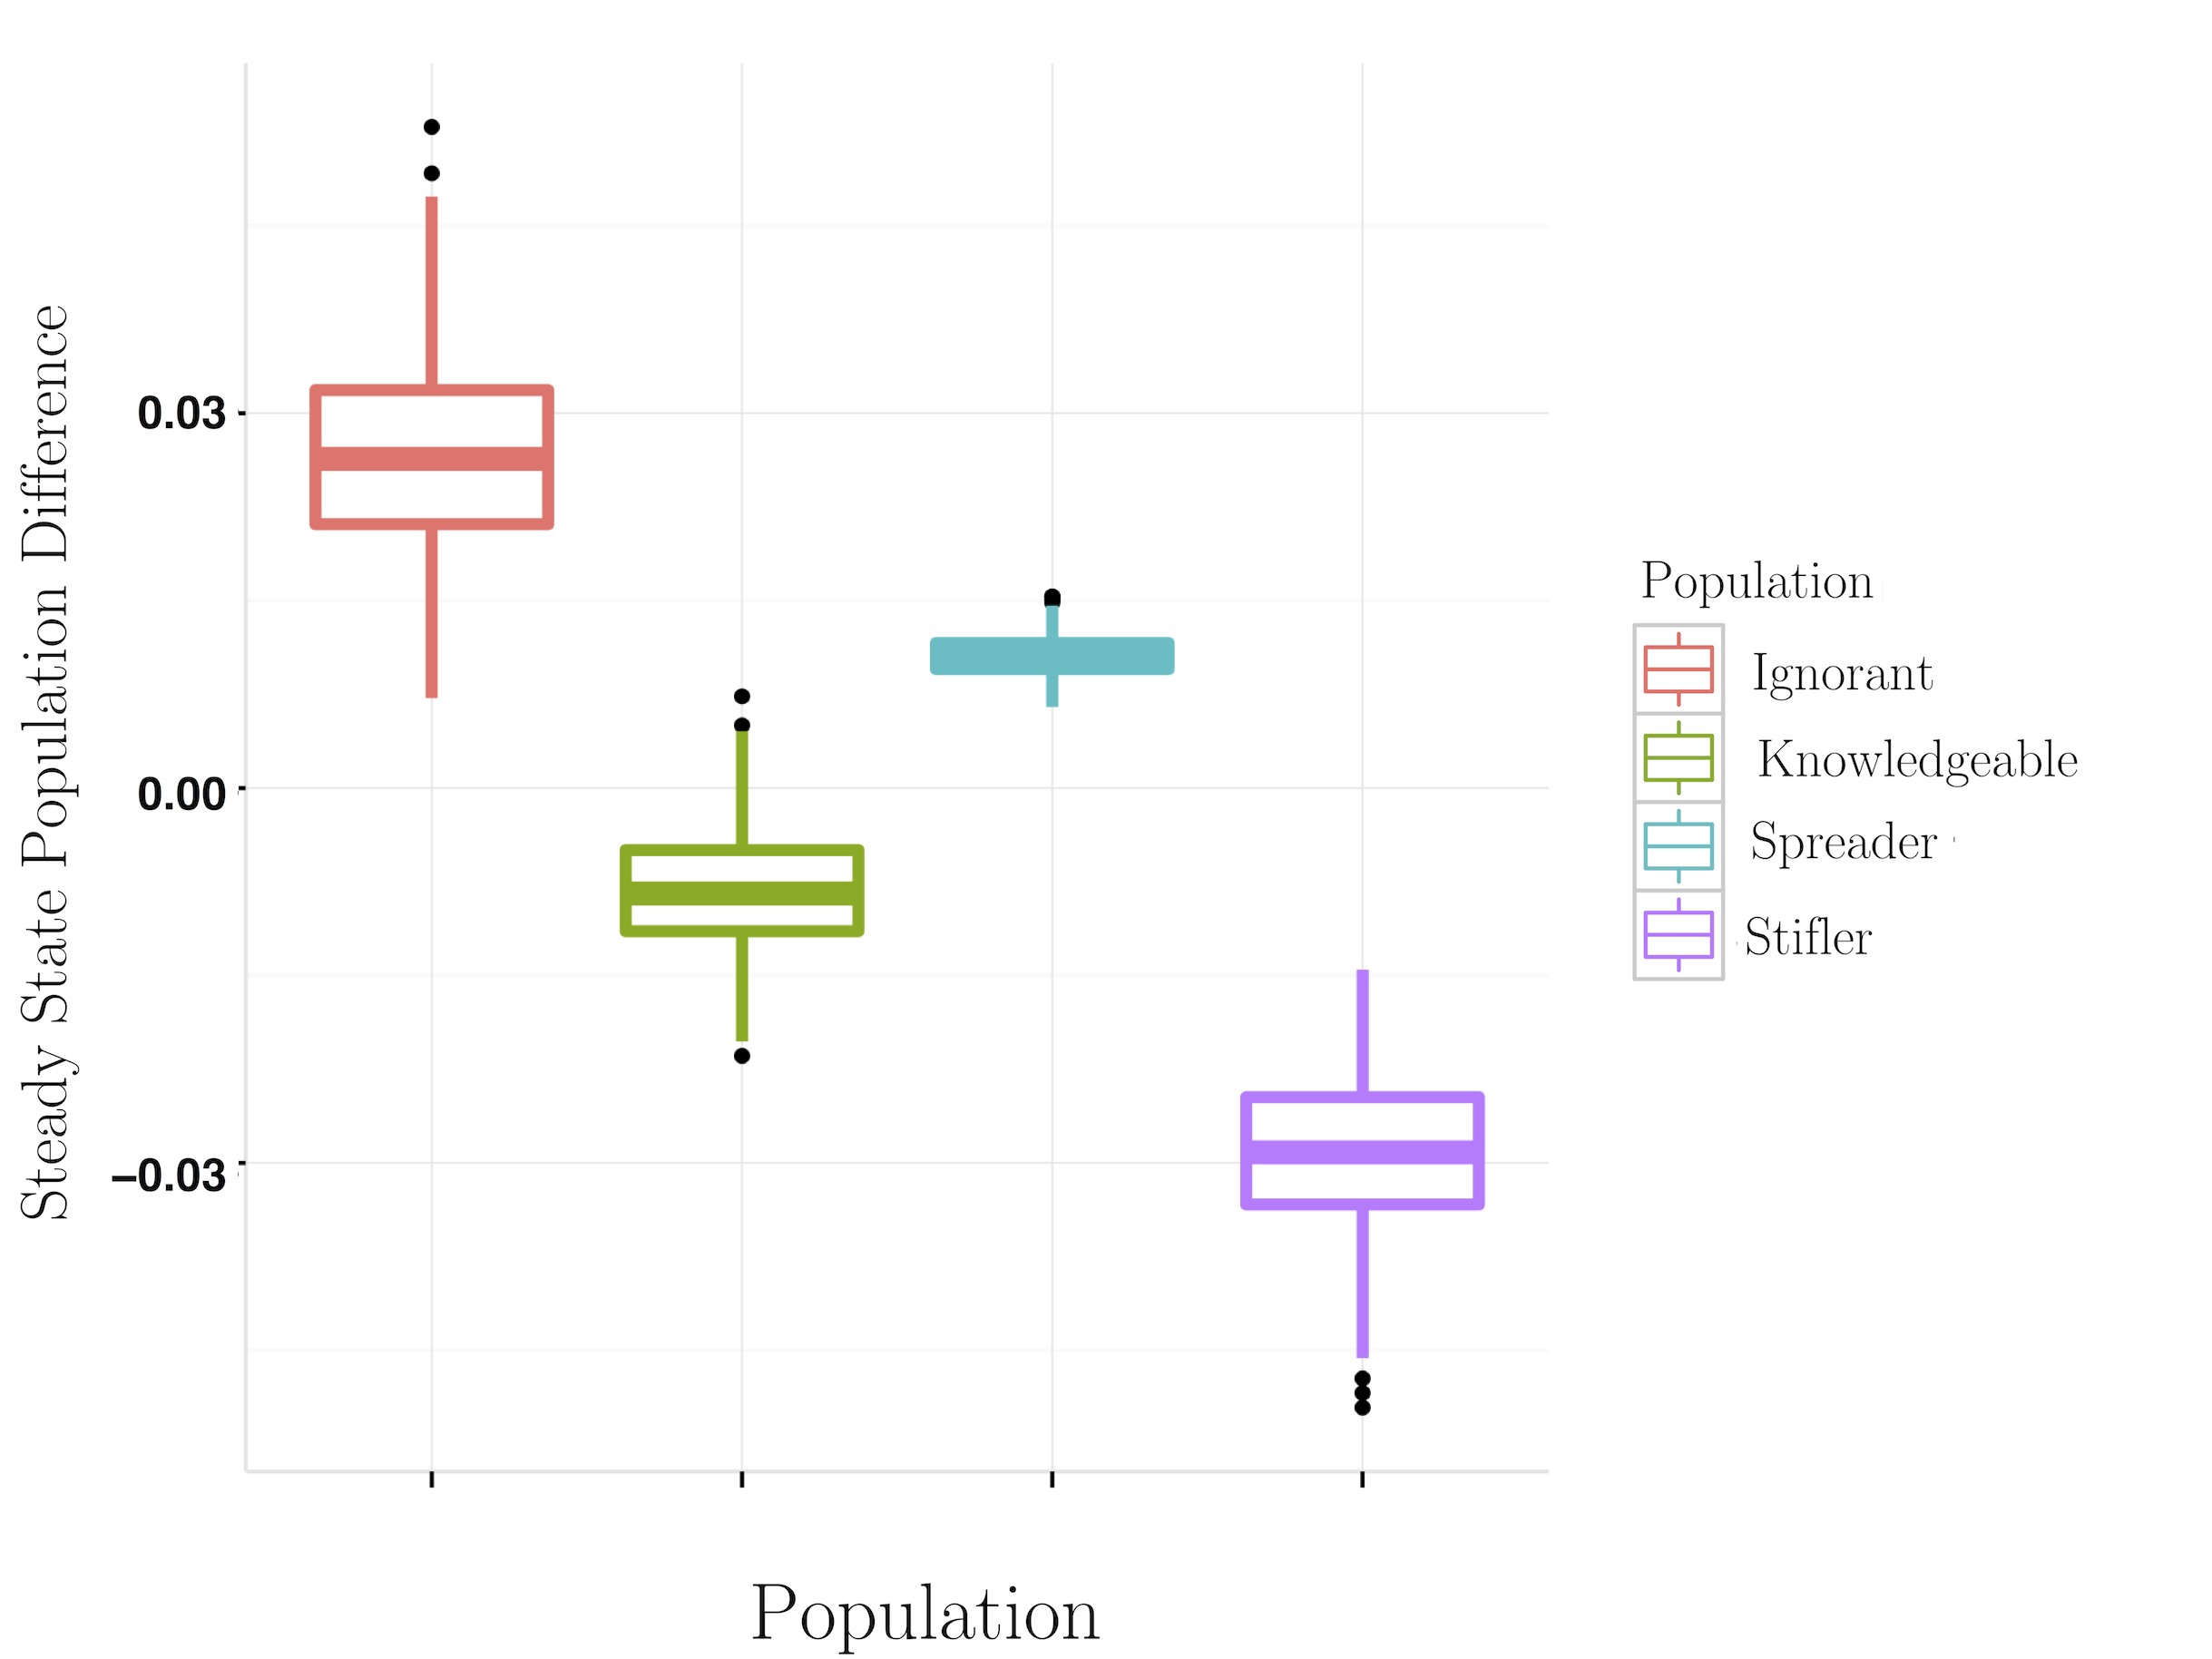
\includegraphics[width=0.7\textwidth]{figures/figure6}
  \caption{Box-and-whisker plot comparing the steady states in the differential model and simple, agent-based model.}
\label{fig:figure6}
\end{figure}

With Figure~\ref{figure:6}, we can directly compare the steady states of the differential model from Figure~\ref{fig:figure1} and the distribution of steady states of the simple, agent-based model from from Figure~\ref{fig:figure6}.
Interestingly, the steady states remain similar, even though the differential model is deterministic, and the simple model incorporates a network.
Both models seem to confirm that eventually, the entire population will be exposed to the rumor, though (as is expected in a stochastic process) the simple model contains very small pockets of ``ignorance.''

\subsection{Feature-Vector, Agent-Based Model}
\label{subsec:featvect}

\begin{figure}[H]
\captionsetup{width=0.8\textwidth}
\centering
    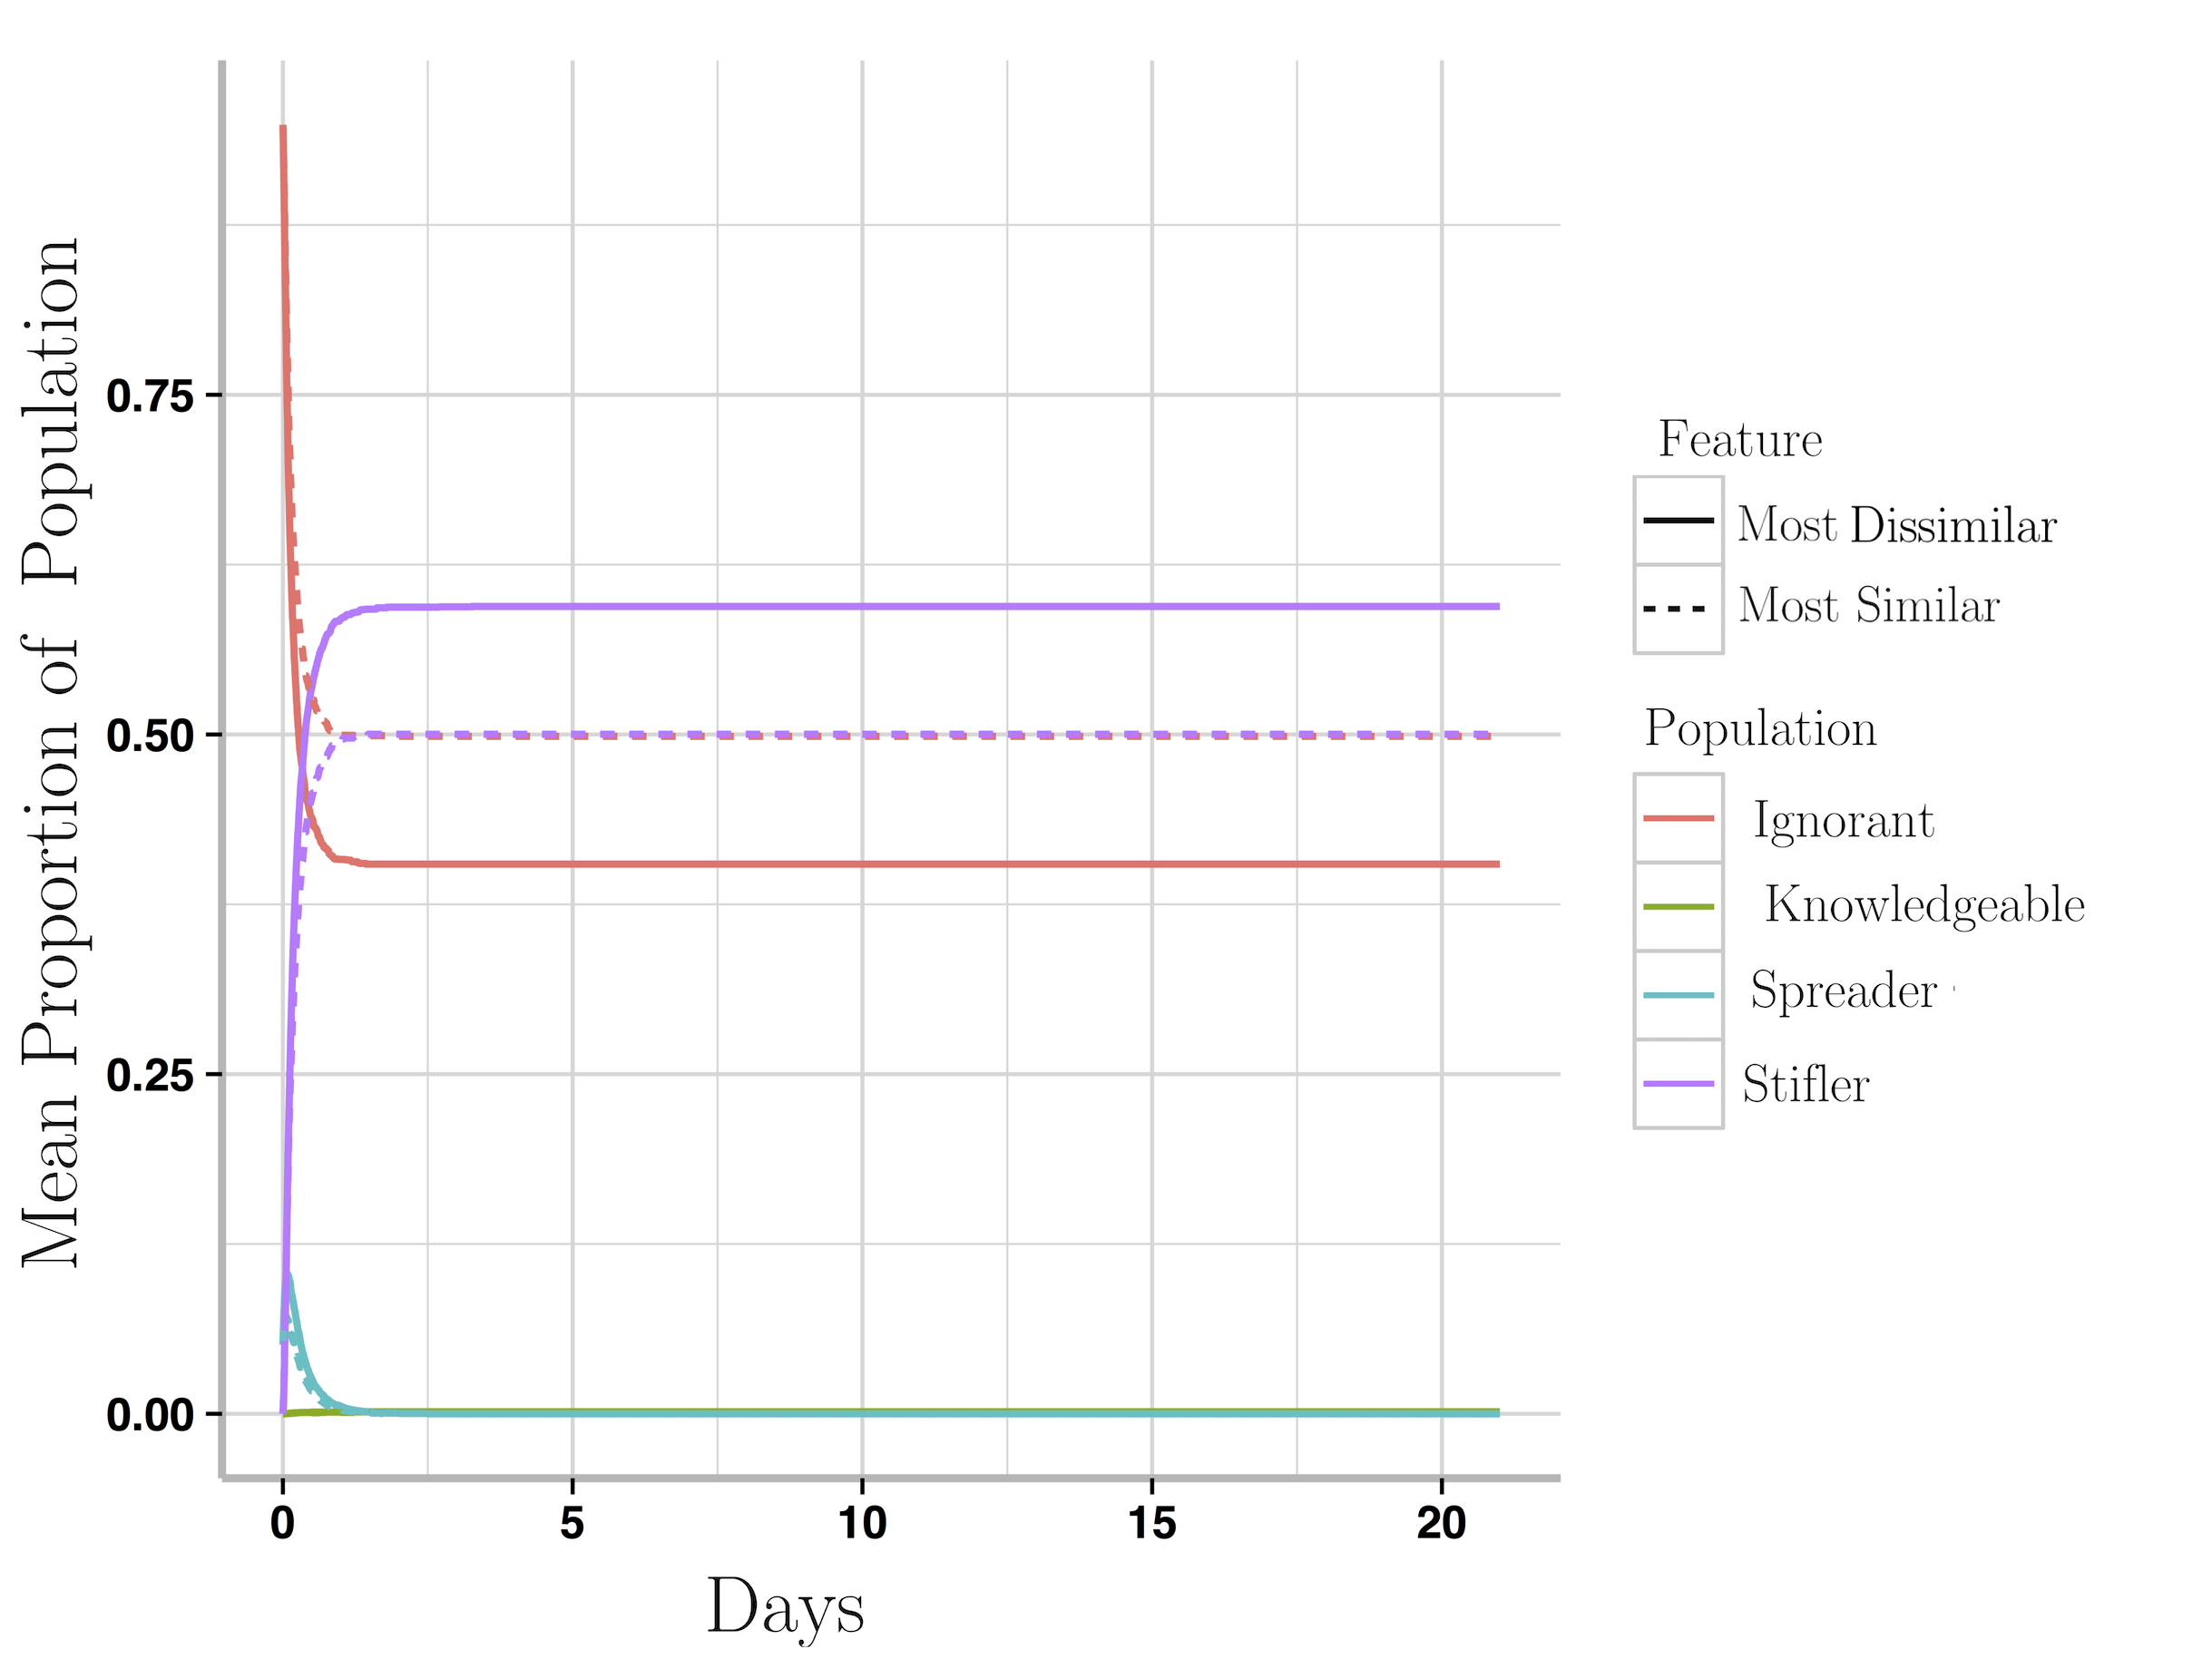
\includegraphics[width=1\textwidth]{figures/figure7}
  \caption{ Results of the most and least similar feature vectors to the population in the agent-based model (average across $ 300 $ trials).}
\label{fig:figure7}
\end{figure}

\begin{figure}[H]
\captionsetup{width=0.8\textwidth}
\centering
    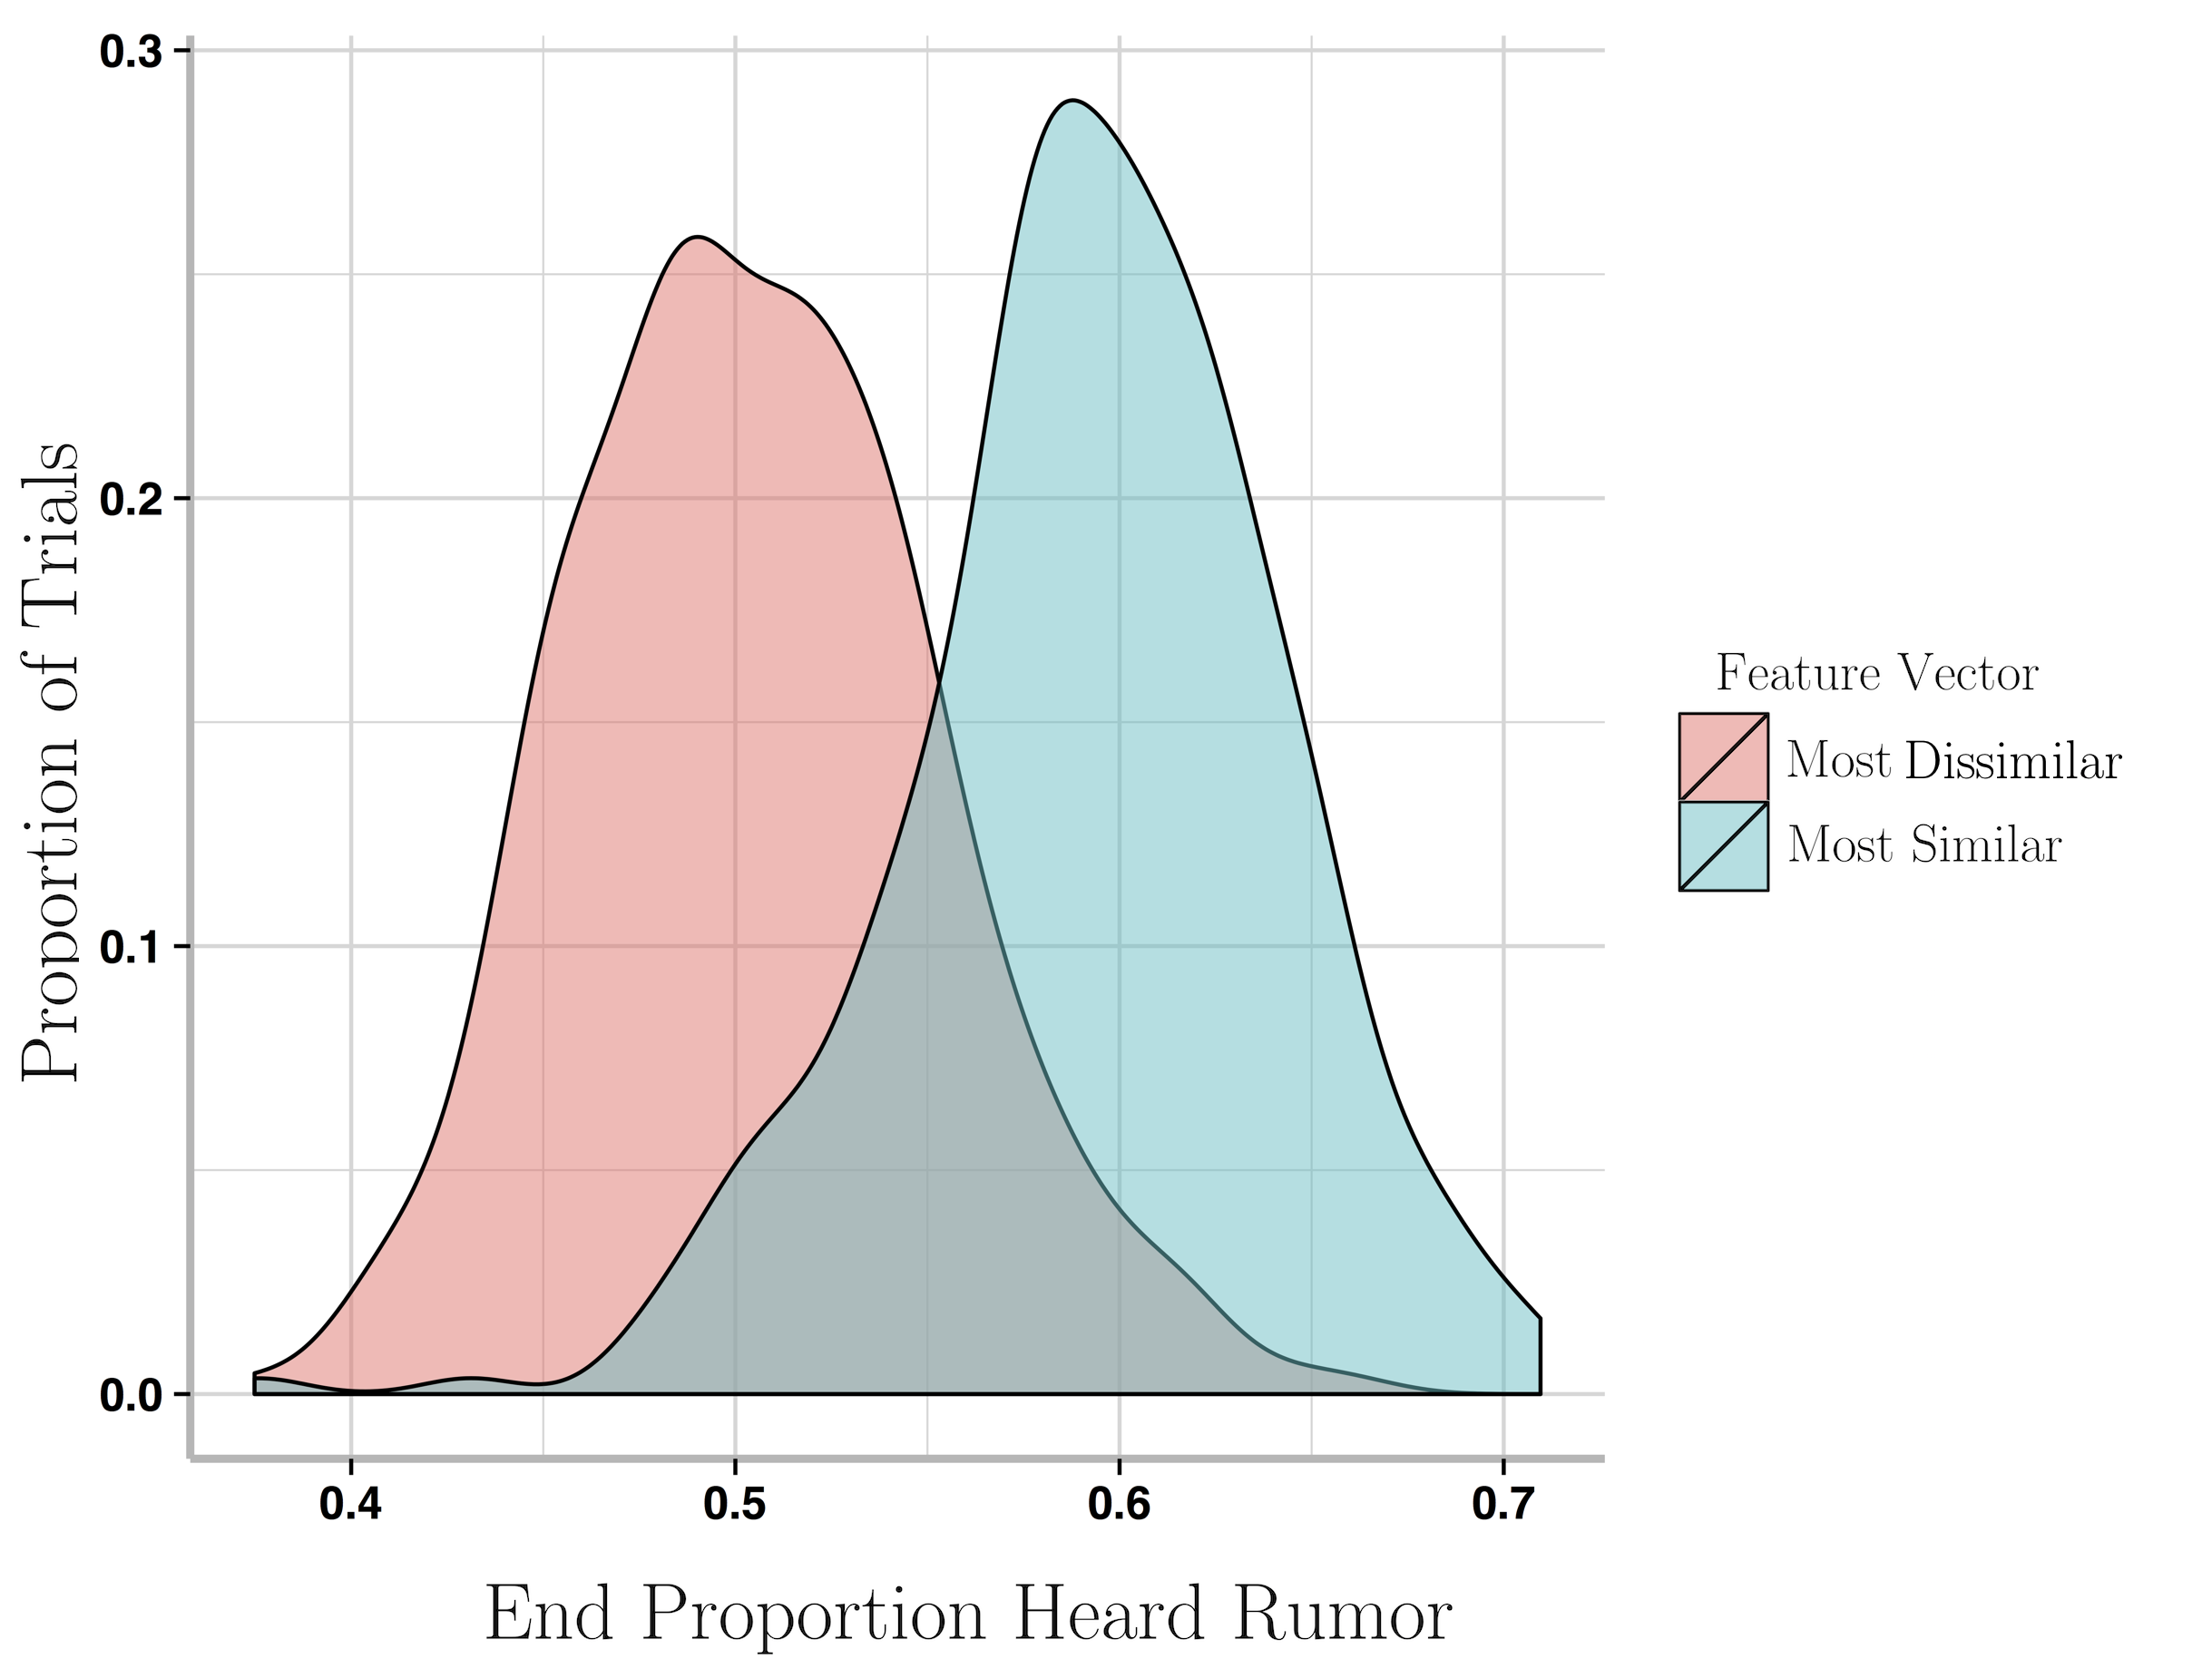
\includegraphics[width=0.7\textwidth]{figures/figure8}
  \caption{ Density of the proportion of the population who heard the rumor after $ 22 $ days with the most and least similar rumors ($ 300 $ trials).}
\label{fig:figure8}
\end{figure}

\begin{figure}[H]
\captionsetup{width=0.8\textwidth}
\centering
    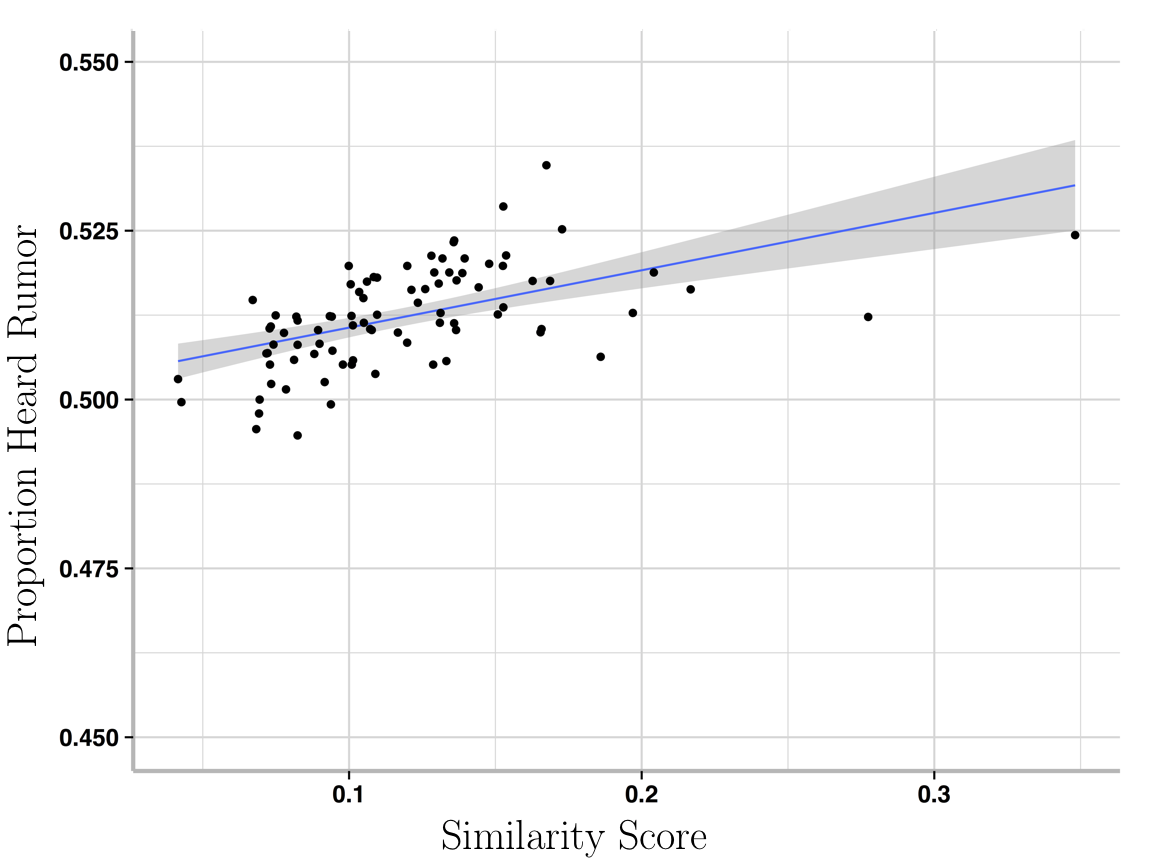
\includegraphics[width=0.7\textwidth]{figures/figure9}
  \caption{ Linear model of the relationship between the final percentage of the population heard rumor and average similarity score of the feature vector ($ r~=~0.538 $).
Shading designates the 95\% confidence interval.}
\label{fig:figure9}
\end{figure}

When the similarity score is added, even the most similar rumor dies out, as seen in Figure~\ref{fig:figure7}.
This plot is identical to Figure~\ref{fig:figure1} and Figure~\ref{fig:figure5}, but is the stochastic agent-based case.
However, the average similarity score of a rumor with the population does affect the spread (Figure~\ref{fig:figure8}).
The most similar rumor to the population spreads to more of the population than does the least similar.
The trend from the other feature vectors supports this claim, as demonstrated by Figure~\ref{fig:figure9}.
The predictive power of the similarity in predicting the number of individuals who heard the rumor is decent where the bulk of the data lies.
